% Standalone System Model Diagram (OAM-FSO)
\documentclass[tikz,border=6pt]{standalone}
\usepackage{amsmath}
\usetikzlibrary{arrows.meta,positioning,fit,shapes.geometric,backgrounds}

\begin{document}
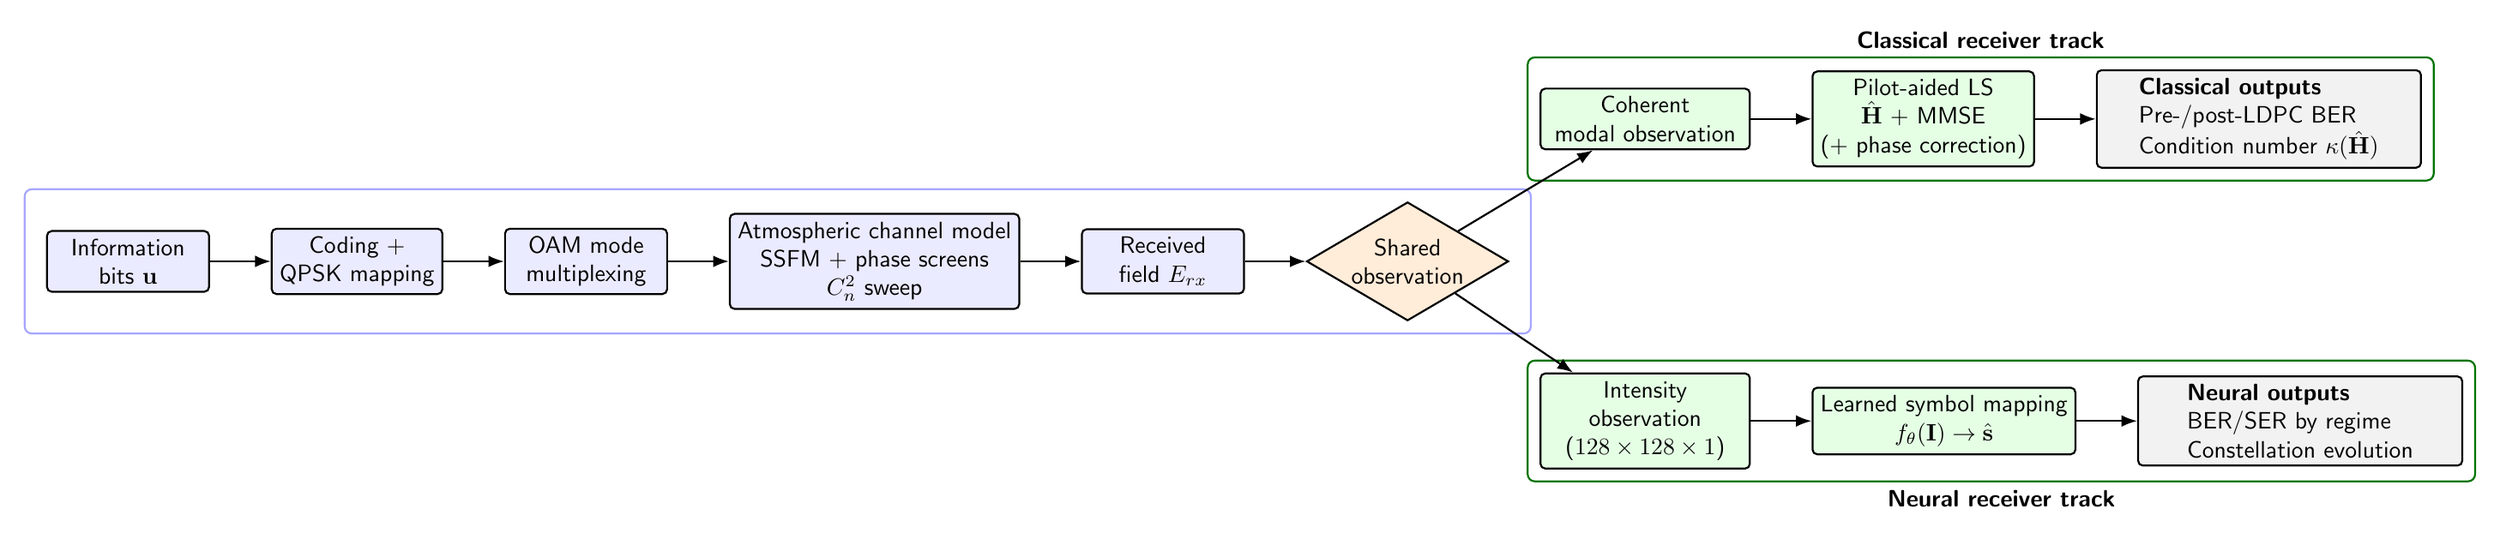
\begin{tikzpicture}[
    font=\sffamily,
    >=Latex,
    node distance=8mm and 9mm,
    block/.style={draw, rounded corners=2pt, thick, align=center, minimum height=8mm, minimum width=24mm, fill=blue!8},
    branch/.style={draw, rounded corners=2pt, thick, align=center, minimum height=8mm, minimum width=28mm, fill=green!10},
    metric/.style={draw, rounded corners=2pt, thick, align=left, minimum height=8mm, minimum width=45mm, fill=gray!10},
    split/.style={diamond, draw, thick, aspect=1.7, align=center, inner sep=1pt, fill=orange!15},
    note/.style={draw, rounded corners=2pt, thick, align=left, minimum width=43mm, fill=yellow!12},
    flow/.style={-Latex, thick}
]

% Shared chain (model-level)
\node[block] (bits) {Information\\bits $\mathbf{u}$};
\node[block, right=of bits] (tx) {Coding +\\QPSK mapping};
\node[block, right=of tx] (oam) {OAM mode\\multiplexing};
\node[block, right=of oam, minimum width=34mm] (chan) {Atmospheric channel model\\SSFM + phase screens\\$C_n^2$ sweep};
\node[block, right=of chan] (rx) {Received\\field $E_{rx}$};
\node[split, right=of rx] (obs) {Shared\\observation};

% Classical branch
\node[branch, above right=12mm and 12mm of obs, minimum width=31mm] (coh) {Coherent\\modal observation};
\node[branch, right=of coh, minimum width=32mm] (mmse) {Pilot-aided LS\\$\hat{\mathbf{H}}$ + MMSE\\(+ phase correction)};
\node[metric, right=of mmse, minimum width=48mm] (cout) {\textbf{Classical outputs}\\Pre-/post-LDPC BER\\Condition number $\kappa(\hat{\mathbf{H}})$};

% Neural branch
\node[branch, below right=12mm and 12mm of obs, minimum width=31mm] (img) {Intensity\\observation\\($128 \times 128 \times 1$)};
\node[branch, right=of img, minimum width=32mm] (fth) {Learned symbol mapping\\$f_{\theta}(\mathbf{I}) \rightarrow \hat{\mathbf{s}}$};
\node[metric, right=of fth, minimum width=48mm] (nout) {\textbf{Neural outputs}\\BER/SER by regime\\Constellation evolution};

% Side notes

% Flows (shared chain)
\draw[flow] (bits) -- (tx);
\draw[flow] (tx) -- (oam);
\draw[flow] (oam) -- (chan);
\draw[flow] (chan) -- (rx);
\draw[flow] (rx) -- (obs);

% Branch flows
\draw[flow] (obs) -- (coh);
\draw[flow] (coh) -- (mmse);
\draw[flow] (mmse) -- (cout);

\draw[flow] (obs) -- (img);
\draw[flow] (img) -- (fth);
\draw[flow] (fth) -- (nout);

% Group boxes (visual guidance)
\begin{scope}[on background layer]
  \node[draw=blue!35, rounded corners=3pt, thick, fit=(bits)(obs), inner xsep=9pt, inner ysep=5pt] {};
  \node[draw=green!45!black, rounded corners=3pt, thick, fit=(coh)(mmse)(cout), inner sep=5pt, label={[align=left]above:\textbf{Classical receiver track}}] {};
  \node[draw=green!45!black, rounded corners=3pt, thick, fit=(img)(fth)(nout), inner sep=5pt, label={[align=left]below:\textbf{Neural receiver track}}] {};
\end{scope}

\end{tikzpicture}
\end{document}
